%
\chapter{Abstraction}

Abstraction is an old business, from the syllogism of Aristotle to the recent machine learning. We are using it every day without notice, it reduces our reductant works, it makes education a viable action, it helps understand. At the same time, abstraction is hard to understand, to this day, I can't really appreciate the true meaning of abstraction, and the fundamental information it tries to convey.

What is think abstractly, that means you think in terms of class, in terms of reduce the tightness being too specific and group things with same criteria and make actions and computations in class and apply the result in one time but works for all terms.

One example here is $(x +y )^8$, what is the coefficient of $x^2y^6$? You may say this is a easy task, but you think it fast because you know all the other terms are same for some measure, that they are differ with different $x^k$ in each instance.

Let's make it even more dramastic:

\begin{example}
  $x^2 + x^10 = a_0 + a_1(x+1) + \cdots + a_9(x+1)^9 + a_10(x+1)^10$, find $a_9$
\end{example}

In this case, if you have to think too specific, you would end up writing long sequence of the terms, while all you need to figure out is that $a_9$

\section{Atomized Abstracion}

Here we are treating abstraction as information, as pieces of information. atomized pieces. builded up as abilities and cares. features and

% introduction
\subsection*{100 Examples of Abstraction}

As I discuss in the distinguishability, this concept is so important and so ubiquitous, I have to do this anonying action again in this book.
\subsection*{Invariance under Variation}
% \subsection{Distinguishability with Abstraction}
% \subsection{Real-Life Examples}
\subsection*{Evolution Perspective}

I always find evolution has its best choice. The way brain works is actually quite flexible when we talk about its ability to solve various jobs and efficient when consider the complex situation human has to deal with.

1. we have hunter and gather.

2. we must act fast.

3. we have to adapt to various enviroments.

4. we don't need to be too smart, only smart enough to pass the genes on.

5. we want to save brain energy in order to live on limited energy available.

Following is my personal guess on evolution and brain functionality:

Let's imagine a situation that we need to survive in wild, we need to hunt and gather food.

The evolutional advantages of brain is to process the information, and so we could separate harm from goods. More and more we gain the ability of not only distinguish one thing to another. But also able to predict the future, which can learn the rules of transformation.

While this is still not that helpful, since we need to be able adapted to a large range of situations. If we understand things too specific, we can't predict the new situation that varies a little bit.

And also in the very beginning of eyes, we could only see a very low resolution of the world, that's an advantage somehow. Since we could only care a low level of certainty to be survive, and when we don't have high level functionality to process and predict. Vague means robost when you have only one technique at hand.

Gradually, brain evoles to a new level that high resolution is helpful and precise descriptions means a precise prediction. But at the same time the old part of the brain remains as a part of function to provide levels of resolutions. That means when we have an image input to our brain, it could be able to store multiple copies of the image, varies in terms of resolution. If we talk in the object oriented programming way, that means we have lots of inherence there.

What I mean here as resolution is not that in graphics, but the resolution of information, to what degree we care about the distinction of two similiar objects.

In high resolution, the details are described precisely. While in low resolution, we consider human and rock both as physical object. In terms of what concerns us, we make different views of things.

Let's take a picture for example:

This is an image with a bowl and some corns. While I see this, the image is not only the rice and corns, it's also a thing with yellow and white.

Resolution means you can distinguish stuff in level of needs, at different context, you need different contrast to solve the problems at hand.

Let us review this part:

First, evolution gives us the ability to distinguish data.

Then, we need to distinguish data with vague, which essentially class level information or abstract information.

Third, not only we predict, but also we need to learn the rule of inference, under what condition, what input will transform to what ouput.

% \subsection{Regular Expression}
% \subsection{Context-Free Grammar}

% Definition
\chapter{Problems}

% introduction
\section{Problems}

To define a problem is defining a class at the same time.

To understand a problem is to know how to check whether one solution is correct or not.
\subsection{Verifying versus Searching}


% types of problems
\section{Types of Problems}
\subsection{Computational Problems}
\subsection{Learning Problems}
\subsection{Generic Problems}

% definition and properties of techniques
\section{Techniques}
The Classification of Techniques is a core concept in daily life.
\begin{figure}
  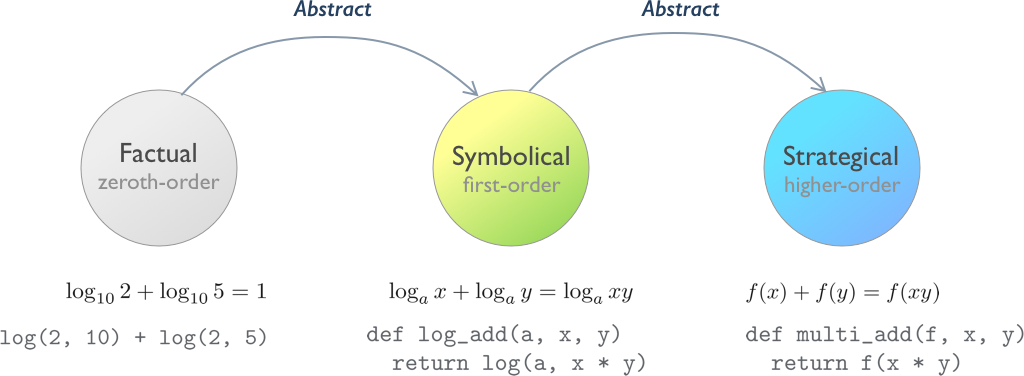
\includegraphics[width=\linewidth]{img/abstract-levels.png}
  \caption{Abstraction Levels}
  \label{fig:abstract-levels}
\end{figure}
\subsection{Robustness of Techniques}
\subsection{Frequency of Usage}
\subsection{Ad-Hoc versus Generic}
One phenominon that I experience a lot is the way people don't distinguish the difference between a ad-hoc technique and a generic technique. When a teacher or a guy present a way to solve a specific problem, few people will appreciate the robustness of this technique, that how well can you transfer your ability on this learning to another situations. But because of their inability to distinguish hardness and robustness, that leads to a dangerous place, that you have to learn too much techniques to cope with every problems, but you don't have enough time for learning these. And the teacher may think by doing an ad-hoc problem will lead to a better understanding for a more generic solving ability, which is vague. You don't learn too much on ad-hoc problems. You only know how to solve it in a nearby situations. The overall hint on a more generic solving strategies are often weak to recognize.

People don't know how to appreciate the robustness of techniques. Only can they find the dramatic changes of events. Even you simply press the button, you believe the underlining changes belongs to your smartness, well the main reason is the engineering behind the scene to smooth the user experience.
\subsection{Intensity of Signal}
\subsection{Trainability of Techniques}
Both the solving radius and the applicability.

% types of techniques
\section{Types of Techniques}
\subsection{Factual Techniques}
\subsection{Algorithmic Techniques}
\subsection{Strategic Techniques}
\subsection{Generic Techniques}
\subsection{Expansion Techniques}


% Generate class from instance and other classes.
\section{Hierarchy of Abstraction}
\subsection{Resolution of Distinguishability}

When you say something about a data. $x^2 + y^2 =1$, what you are getting is that you are saying some truth about $(x,y)$, how to distinguish them from others, and how to use it as a way to generate the feature of this point, to use it as a weapon, to find facts that is also true for little $(x, y)$
\subsection{Hierarchy of Formal Languages}
\subsection{Pattern Recognization}
\subsection{Feature Extraction}

% compositions
\section{Composition with Abstraction}

% class level transformation
\section{Transformation with Abstraction}
\subsection{Confident Extrapolate}
\subsubsection*{From one instance to whole class}

\begin{figure}
  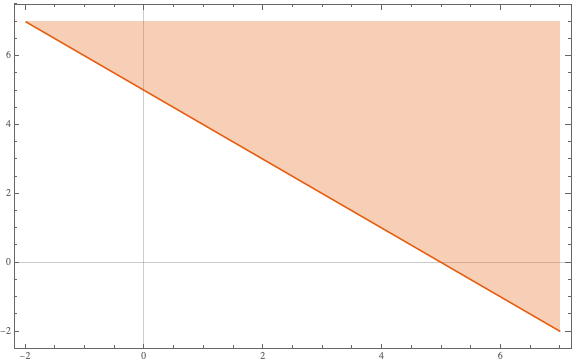
\includegraphics[width=\linewidth]{img/5-x.png}
  \caption{Plof of $ x + y \geqslant 5$}
  \label{fig:5-x}
\end{figure}

To determine which part is $ x + y \geqslant 5$, upper or lower of $ x + y = 5$, we only need to plug in a number that is not on the line, say $(0, 0)$, since $0+ 0 \ngeqslant 5$, we can deduce that the shaded area should be the upper part of the image, as shown in Figure \ref{fig:5-x} This single one instance is sufficient to represent the whole class, in this case we can use one to proof the all.

\subsubsection*{From several instances to whole class}

\chapter{Problems}

% introduction
\section{Problems}

To define a problem is defining a class at the same time.

To understand a problem is to know how to check whether one solution is correct or not.
\subsection{Verifying versus Searching}


% types of problems
\section{Types of Problems}
\subsection{Computational Problems}
\subsection{Learning Problems}
\subsection{Generic Problems}

% definition and properties of techniques
\section{Techniques}
The Classification of Techniques is a core concept in daily life.
\begin{figure}
  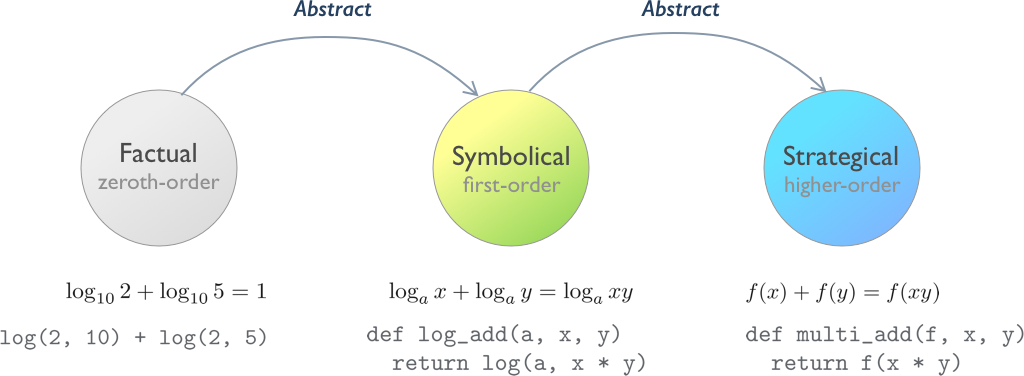
\includegraphics[width=\linewidth]{img/abstract-levels.png}
  \caption{Abstraction Levels}
  \label{fig:abstract-levels}
\end{figure}
\subsection{Robustness of Techniques}
\subsection{Frequency of Usage}
\subsection{Ad-Hoc versus Generic}
One phenominon that I experience a lot is the way people don't distinguish the difference between a ad-hoc technique and a generic technique. When a teacher or a guy present a way to solve a specific problem, few people will appreciate the robustness of this technique, that how well can you transfer your ability on this learning to another situations. But because of their inability to distinguish hardness and robustness, that leads to a dangerous place, that you have to learn too much techniques to cope with every problems, but you don't have enough time for learning these. And the teacher may think by doing an ad-hoc problem will lead to a better understanding for a more generic solving ability, which is vague. You don't learn too much on ad-hoc problems. You only know how to solve it in a nearby situations. The overall hint on a more generic solving strategies are often weak to recognize.

People don't know how to appreciate the robustness of techniques. Only can they find the dramatic changes of events. Even you simply press the button, you believe the underlining changes belongs to your smartness, well the main reason is the engineering behind the scene to smooth the user experience.
\subsection{Intensity of Signal}
\subsection{Trainability of Techniques}
Both the solving radius and the applicability.

% types of techniques
\section{Types of Techniques}
\subsection{Factual Techniques}
\subsection{Algorithmic Techniques}
\subsection{Strategic Techniques}
\subsection{Generic Techniques}
\subsection{Expansion Techniques}


\subsection{Analogy}

% class level computation
\chapter{Problems}

% introduction
\section{Problems}

To define a problem is defining a class at the same time.

To understand a problem is to know how to check whether one solution is correct or not.
\subsection{Verifying versus Searching}


% types of problems
\section{Types of Problems}
\subsection{Computational Problems}
\subsection{Learning Problems}
\subsection{Generic Problems}

% definition and properties of techniques
\section{Techniques}
The Classification of Techniques is a core concept in daily life.
\begin{figure}
  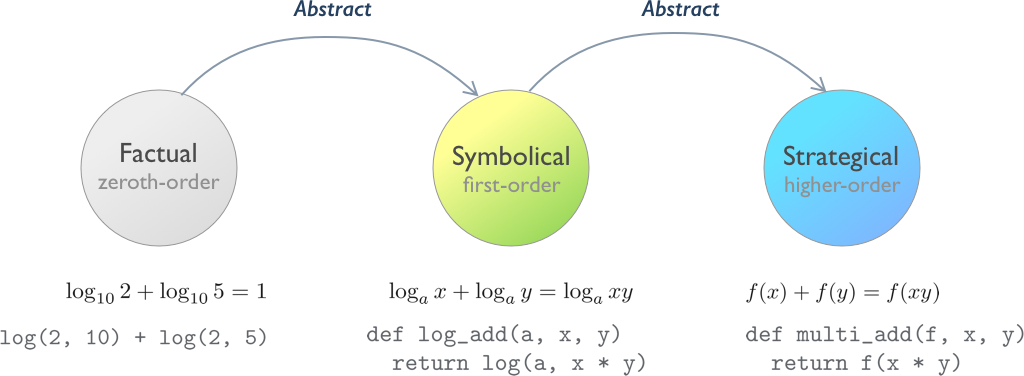
\includegraphics[width=\linewidth]{img/abstract-levels.png}
  \caption{Abstraction Levels}
  \label{fig:abstract-levels}
\end{figure}
\subsection{Robustness of Techniques}
\subsection{Frequency of Usage}
\subsection{Ad-Hoc versus Generic}
One phenominon that I experience a lot is the way people don't distinguish the difference between a ad-hoc technique and a generic technique. When a teacher or a guy present a way to solve a specific problem, few people will appreciate the robustness of this technique, that how well can you transfer your ability on this learning to another situations. But because of their inability to distinguish hardness and robustness, that leads to a dangerous place, that you have to learn too much techniques to cope with every problems, but you don't have enough time for learning these. And the teacher may think by doing an ad-hoc problem will lead to a better understanding for a more generic solving ability, which is vague. You don't learn too much on ad-hoc problems. You only know how to solve it in a nearby situations. The overall hint on a more generic solving strategies are often weak to recognize.

People don't know how to appreciate the robustness of techniques. Only can they find the dramatic changes of events. Even you simply press the button, you believe the underlining changes belongs to your smartness, well the main reason is the engineering behind the scene to smooth the user experience.
\subsection{Intensity of Signal}
\subsection{Trainability of Techniques}
Both the solving radius and the applicability.

% types of techniques
\section{Types of Techniques}
\subsection{Factual Techniques}
\subsection{Algorithmic Techniques}
\subsection{Strategic Techniques}
\subsection{Generic Techniques}
\subsection{Expansion Techniques}

